% TeX encoding = utf8
% TeX spellcheck = en 

% Piotr Zdunek - Master Thesis 
\documentclass{pzdunek_master_thesis}
\usepackage[english]{babel}
%\usepackage{polski}
\usepackage{graphicx}
\usepackage{caption}
\usepackage{subcaption}
\usepackage{amsfonts}
\usepackage{amsmath}
\usepackage{amsthm}
\usepackage{wrapfig}
\usepackage{listings}
\lstset{language=C}
\usepackage{moreverb}
\usepackage{booktabs}
\usepackage{eurosym}
\usepackage{indentfirst}
\usepackage{pdfpages}
\usepackage[utf8]{inputenc}
\usepackage{enumitem}
\usepackage{multirow}
\usepackage{rotating}
\usepackage{float}
\usepackage{tocloft}
\usepackage{color}
\usepackage{mathtools}
\usepackage{setspace}\setstretch{1.2}
\usepackage{tabularx}
\usepackage{tgtermes}
\usepackage[titletoc]{appendix}
\usepackage{booktabs}
\usepackage{enumitem}
\setlist[1]{itemsep=-5pt}
\newcommand{\ra}[1]{\renewcommand{\arraystretch}{#1}}
\usepackage{color, colortbl}
\usepackage{array}
\usepackage{ragged2e}
\newcolumntype{P}[1]{>{\RaggedRight\hspace{0pt}}p{#1}}
\usepackage{footnote}
\usepackage{ctable}
%no borders around hyperlinks
\usepackage{hyperref}
\hypersetup{%
    pdfborder = {0 0 0}
}

\usepackage[nonumberlist,nopostdot]{glossaries}
\deftranslation{Glossary}{Glossary}
\newcommand{\dictentry}[2]{%
  \newglossaryentry{#1}{name=#1,description={#2}}%
  \glslink{#1}{}%
  \glsgroupskip
}%
\makeglossaries
\cleardoublepage

%\author{\Huge\href{p.zdunek@stud.elka.pw.edu.pl}{\textbf{Piotr Zdunek}}}
\nralbumu{229417}
\title{High speed multichannel camera with 10 GbE}

%\tytulang{The aim of this Master Thesis was to design a high performance }
  
%\kierunek{Microsystems and electronics systems}

%\titlepl{Szybka wielokanałowa kamera z interfejsem 10 GbE}

%\abs_text{Poniższa praca przedstawia opis projektu oprogramowania na kamerę. }

%\keywords{Camera, ZYNQ, FPGA, Scientific, Framework}

% miesi?c i rok
\date{Warsaw, 2015}

% koniec definicji

\begin{document}
%\def\tablename{Tabela}%
\maketitle
%\tableofcontents
%\newpage
%\listoffigures
%\listoftables
%\clearpage

\dictentry{BGA}{Ball Grid Array}
\dictentry{CMOS}{Complementary Metal-Oxide Semiconductor} 
\dictentry{PCIe}{ Peripherial Component Interconnect Express }
\dictentry{GTP}{Gigabit Transceiver Port}
\dictentry{AC}{Alternating Current}
\dictentry{DC}{Direct Current}
\dictentry{FPGA}{Field Programmable Gate Array}
\dictentry{IC}{Integrated Circuit}
\dictentry{JTAG}{Joint Test Action Group}
\dictentry{DDR}{Double Data Rate}
\dictentry{PCB}{Printed Circuit Board}
\dictentry{PERG}{Photonics and Web Engineering Group}
\dictentry{SFP+} {Small form-factor pluggable transceiver}
\dictentry{Gbps} {Gigabits per second}
\dictentry{GFLOPs} {Giga Floating Point Operations Per Second}
\dictentry{SPI} {Serial Peripherial Interconnect}
\dictentry{I2C} {Inter Integrated Circuit}
\dictentry{ppm} {points per milion}
\dictentry{LVDS} {Low Voltage Differential Signaling}
\dictentry{GB} {Gigabyte}
\dictentry{EDA} {Electronic Design Automation}
\dictentry{OHWR} {Open Hardware Repository}
\dictentry{TTM} {Time To Market}
\dictentry{SoC} {System-On-Chip}
\dictentry{PC}	{Personal Computer}
\dictentry{GPU}	{Graphics Processing Unit}
\dictentry{GPGPU}	{General Purpose Graphics Processing Unit}
\glsnogroupskiptrue
\clearpage
\printglossary[style=index]
\clearpage

%----------------------------------------------------------------------------------------------------------
%Introduction
\chapter{Introduction}
\label{chapt:introduction}

\chapter{Introduction}

\lipsum[3-56]
\section{Project genesis}
\section{Motivation and Objectives}
\subsection{Literature review}
\subsection{Market review} 
\section{Requirements}
%Compact, low weight, high speed, two different sensors, rugged
\section{Thesis statement} 
%Make an embedded camera and evaluate the use of high-speed interfaces for hyper-spectral aerial applications. 


%----------------------------------------------------------------------------------------------------------
%GENEZA, CEL, ZAŁOŻENIA
\chapter{Genesis, goals and assumptions}
\label{chapt:genesis}
\chapter{Genesis}

In this master thesis an implementation of Precision-Time-Protocol Timestamping Unit in FPGA fabric for scientific
camera systems is presented. The project was completed at Photonics and Web Engineering Group at the Institute of 
Electronics Systems which has a significant contribution to X-ray measurement research (TODO publikacje).  Having a scientific cooperation with
another Polish university, there was a need to develop hardware and firmware for novel extremely high-speed,
multichannel, X-ray silicon based camera. This project is undergoing a patent application, and for this reason the 
detailed description of the project cannot be included in this thesis. 

Specifically, a time synchronisation system providing an accurate UTC time was required in order to correctly control
the exposure time between the systems' channels.  This master thesis focuses on that aspect of the project.   


\section{Problem statement}
Providing an accurate timestamping for modern scientific grade camera system is a \textbf{complicated engineering
problem}. The designed hardware for the camera system used Xilinx Zynq SoC\cite{XIL:ZYNQ} which has built
in timestamping capability in the Media Access Controller (MAC). Nevertheless, the timestamping register is not available for
to be read by the operating system and programmable logic \cite[16.4.2]{XIL:ZYNQ_TRM} and the provided functionality of timestamping from
Xilinx is limited and provides low accuracy \cite[16.2.7]{XIL:ZYNQ_TRM} and significant jitter \cite{XIL:PTP_TESTS}. 
Xilinx User Guide Number 585 - Technical Rerence Manual explicitly mentions the fact that the Timestamping Unit can be 
implemented in hardware (programmable logic) in order to achieve better accuracy. This has not been done before and 
this thesis provides the solution to the mentioned problem. 

\section{Solution}
The solution for the problem is to design a Timestamping Unit (TSU) in digital system in FPGA fabric for the Zynq SoC
and use the MAC's built in PTP filtering capability to use this IP Core as a replacement for the internal built in TSU.
What is more, an Ethernet driver modification is required to exchange the TSU and an external oscillator has to be added
to the system in order to precisely run the counters in the TSU. 

\section{Statement of Originality}

This solution provides a way to perform PTP based time synchronisation using Zynq SoC. There are
other methods which provide time synchronisation of different precision such as:
\begin{itemize}
    \item GPS
    \item NTP - precision of up to
    \item PTP (by standard) - sub-milisecond precision 
    \item White Rabbit - sub-nanosecond precision 
\end{itemize}

Nevertheless, the solution provided in this master thesis is \textbf{original}. Standard PTP in the
Zynq SoC does not function properly and in order to be able to use PTP on Zynq with high precision and low jitter,
TSU needs to be implemented in digital fabric.  



%----------------------------------------------------------------------------------------------------------
%KONCEPCJA
\chapter{Concept of realisation}
\label{chapt:concept}
\chapter{Concept of design}
In this chapter a concept of the design of the camera is presented. First of all, main camera requirements are shown and juxtaposed with possible solutions. Afterwards the specification of the design is described in detail.

\section{Main requirements}

\begin{itemize}
\item Framerate at 100 fps at 2048 x 2048 resolution
\item High speed interface 
\item Processing capability
\item Possible IMU integration
\end{itemize}

\section{Specification}

\begin{itemize}
\item Framerate at 180 fps at 2048 x 2048 resolution
for CMV4000 and 100 fps for CIS1910F
\item 6.25 Gbps interfaces: SDI, CoaXPress, Aurora, PCie
\item FPGA fabric for processing ability
\item RS485 for communication with IMU and master controller

\end{itemize}


%----------------------------------------------------------------------------------------------------------
\chapter{Realisation}

\section{Firmware}
\label{chapt:realisation}
\input{./chap/sw.tex}

\section{Digital system design}
\label{chapt:fpga}
\input{./chap/fpga.tex}

%----------------------------------------------------------------------------------------------------------
\chapter{Tests}
\label{chapt:Tests}
\chapter{Tests}
\label{ch6:tests}

This chapter presents tests carried out in order to verify the proper working of the realised framework. 
%In order to test the developed framework a new hardware was used with a dedicated sensor. 

%Hardware and sensor was provided by Creotech Instruments S.A. which was developing a scientific camera with cooperation with Cracow University
%of Technology. The framework was adapted to the new hardware and acquisition from the dedicated sensor was performed
%using one of the before mentioned techniques. 


\section{Custom Silicon Sensor - Ethernet data transmission}

\subsection{Setup}
\subsection{Test results}


\section{CMV4000 - Serial ATA SSD video data storage}

\subsection{Setup}
The development system was configured with CMV4000 acquisition IP and Serial ATA. The video data correctness was tested
using Ethernet interface which was sensing acquired frames using RTP\footnote{Real-Time Transport} protocol. 

\subsection{Test results}
Video data reception from the CMV4000 CMOSIS sensor was successful. Figure~\ref{PIC:OUTPUT0} presents the acquired image
of the fan which was used for testing the speed of the camera reception.

\begin{figure}[H]
    \centering
    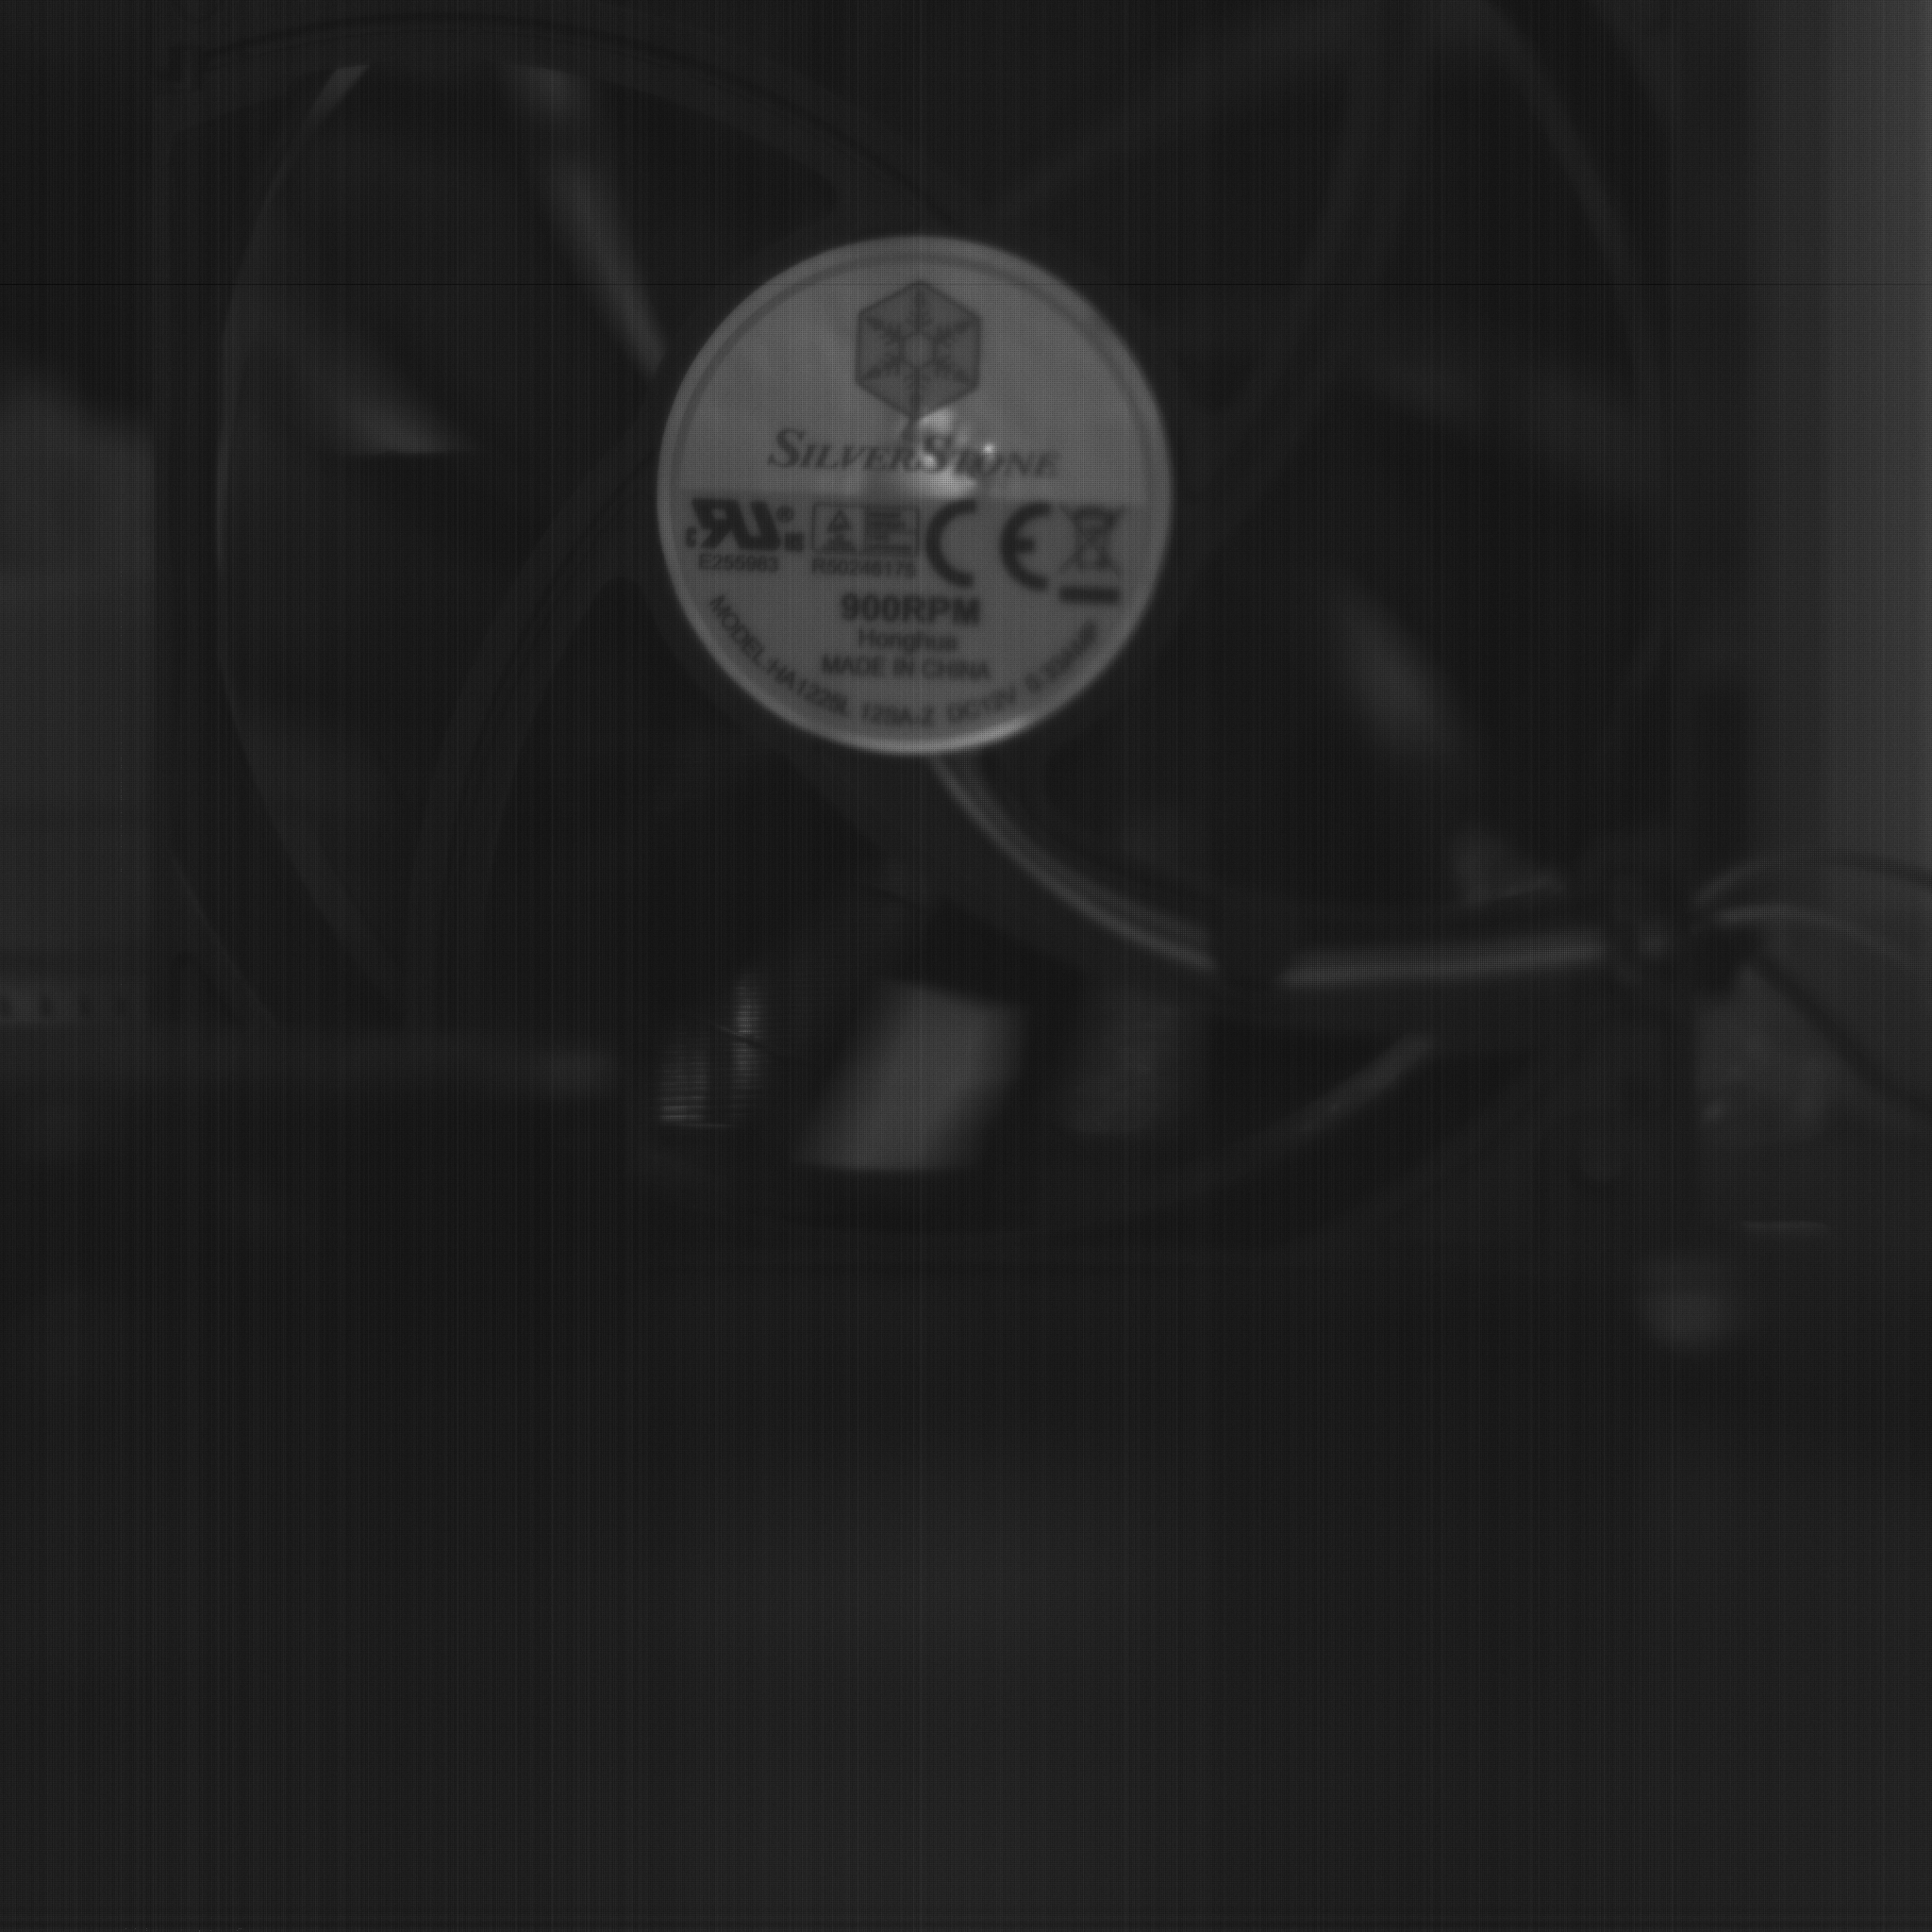
\includegraphics[width=13cm]{img/tests/output0.png}
    \caption{Acquired image from the CMV4000 sensor}
    \label{FIG:OUTPUT0}
\end{figure}


Unfortunately the SSD data acquisition was unreliable. Small portions of data were possible to be written to both of the
hard drives, nevertheless the IP Core constantly lost communication and was resetting itself. As it turned out, the
reason for that was an interal mechanism for sustaining the \textbf{Link-Up} signal high. This signal, when it is high,
indicated that the calibration of the IP Core was successful and that the data can be written or read. The internal
mechanism detected the state of this signal and in a situation where the signal was low, an \textbf{internal reset} was
performed, which \textbf{disrupted} the video data storing. 


\section{Summary}

As far as testing of the camera framework is concerned, the results partially fulfil the requirements, but more work
has to be performed in order to mitigate the limited performance and functionality in some aspects. These limitation
result mainly in wrong assumptions in terms of correctness of operation of some IP Cores which was not possible to
foresee before development. This also underlines a crucial aspect of embedded system design, that before a hypothesis is
not tested and verified, one can not be certain whether some design works or not. 

The most important functions of the framework work correctly and provide a valuable foundation for camera development.  





%----------------------------------------------------------------------------------------------------------
\chapter{Summary}
\label{chapt:remarks}
\chapter{Summary}


%DODATKI
\begin{appendices}
\label{chapt:appendix}
% TeX encoding = utf8
% TeX spellcheck = pl_PL

\chapter{CD-ROM}

\label{CDROM}

\begin{itemize}

    \item test
\end{itemize}







\end{appendices}
%BIBLIOGRAFIA / LITERATURA
%----------------------------------------------------------------------------------------------------------
\bibliographystyle{unsrt}
\bibliography{bib}
\addcontentsline{toc}{chapter}{Bibliography}
\end{document}

